\ExplSyntaxOn

\int_new:N \l__binp_int
\int_set:Nn \l__binp_int {4}
\tl_new:N \l__bina_tl
\tl_new:N \l__binb_tl
\tl_new:N \l__binhw_tl
\int_new:N \l__bina_int
\int_new:N \l__binb_int
\int_new:N \l__binc_int
\int_new:N \l__bind_int
\fp_new:N \l__bina_fp

\DeclareDocumentCommand \BinaryPrecision {m}
{
  \int_set:Nn \l__binp_int {#1}
}

\cs_new_nopar:Npn \int_to_bin:Nn #1#2
{
  \tl_clear:N #1
  \int_set:Nn \l__bina_int {#2}
  \prg_replicate:nn {\l__binp_int}
  {
    \int_set:Nn \l__binb_int {\int_mod:nn {\l__bina_int} {2}}
    \tl_put_left:Nx #1 {\int_use:N \l__binb_int}
    \int_set:Nn \l__bina_int {\int_div_truncate:nn {\l__bina_int} {2}}
  }
}

\cs_new_nopar:Npn \bin_hamming_weight:NN #1#2
{
  \tl_set_eq:NN \l__binhw_tl #2
  \tl_replace_all:Nnn \l__binhw_tl {0} {}
  \int_set:Nn #1 {\tl_count:N \l__binhw_tl}
}

\cs_new_nopar:Npn \bin_flip_one:NNn #1#2#3
{
  \tl_set_eq:NN #2#1
  \prg_replicate:nn {#3 - 1}
  {
    \tl_replace_once:Nnn #2 {1} {a}
  }
  \tl_replace_once:Nnn #2 {1} {0}
  \tl_replace_all:Nnn #2 {a} {1}
}

\DeclareDocumentCommand \HammingWeight {m m}
{
  \int_to_bin:Nn \l__binhw_tl {#2}
  \bin_hamming_weight:NN #1 \l__binhw_tl
}

\DeclareDocumentCommand \HyperCube {m}
{
  \int_set:Nn \l__binp_int {#1}
  \int_zero_new:c {l__hyper_0_int}
  \int_set:cn {l__hyper_0_int} {-1}
  \int_step_inline:nnnn {1} {1} {#1}
  {
    \int_zero_new:c {l__hyper_##1_int}
    \int_set:cn  {l__hyper_##1_int} {\int_use:c {l__hyper_\int_eval:n {##1 - 1}_int} * (#1 - ##1 + 1) / ##1}
  }
  \fp_set:Nn \l__bina_fp {2^{#1}-1}
  \int_set:Nn \l__binc_int {\fp_to_int:N \l__bina_fp}
  \int_step_inline:nnnn {0} {1} {\l__binc_int}
  {
    \int_to_bin:Nn \l__bina_tl {##1}
    \bin_hamming_weight:NN \l__binb_int \l__bina_tl
    \node[every~ hypercube~ label/.try] (hg- \l__bina_tl) at (\int_use:c {l__hyper_\int_use:N \l__binb_int _int},\int_use:N \l__binb_int) {\texttt{\l__bina_tl}};
    \int_incr:c {l__hyper_\int_use:N \l__binb_int _int}
    \int_incr:c {l__hyper_\int_use:N \l__binb_int _int}
  }
  \int_step_inline:nnnn {0} {1} {\l__binc_int}
    {
      \int_to_bin:Nn \l__bina_tl {##1}
      \bin_hamming_weight:NN \l__binb_int \l__bina_tl
      \int_step_inline:nnnn {1} {1} {\l__binp_int}
      {
        \bin_flip_one:NNn \l__bina_tl \l__binb_tl {####1}
        \tl_if_eq:NNTF \l__bina_tl \l__binb_tl
          { % do nothing if nodes are the same
          }
          {
            \draw[every~ hypercube~ edge/.try] (hg- \l__bina_tl) -- (hg- \l__binb_tl);
          }
      }
    }
  }

\ExplSyntaxOff

% Macro to cross out a single node
\newcommand{\CrossOutNode}[1]{%
  \draw[red, thick]
    ($(#1) + (-0.3, 0.3)$)
    --
    ($(#1) + (0.3, -0.3)$);
  \draw[red, thick]
    ($(#1) + (-0.3, -0.3)$)
    --
    ($(#1) + (0.3, 0.3)$);
}

% Macro to cross out a list of nodes
\newcommand{\CrossOutNodes}[1]{%
  \foreach \n in {#1} {%
    \CrossOutNode{\n}%
  }
}
% Macro to draw a circle around a single node
\newcommand{\CircleNode}[2][RoyalBlue]{%
  \draw[#1, thick]
    ($(#2)$)
    circle (0.5);
}

% Macro to circle a list of nodes
\newcommand{\CircleNodes}[2][RoyalBlue]{%
  \foreach \n in {#2} {%
    \CircleNode[#1]{\n}%
  }
}

% Überwachungstabelle der Aufgabe mit 10 Nachrichtenbits und 4 Kontrollbits
% (Spalten 1 bis 14, Zeilen c1 bis c4); Massstab im tikzpicture setzen
\newcommand{\ueberwachungZehnVier}{%
  \fill[blue!25] (0,0) rectangle (15,1);
  \fill[blue!15] (0,-4) rectangle (1,0);
  \fill[gray!8] (1,-4) rectangle (15,0);
  \foreach \i in {1,...,10} {
      \node at (\i+.5,.5) {\(a_{\i}\)};
    }
  \foreach \i in {1,...,4} {
      \pgfmathtruncatemacro{\col}{10+\i}
      \node[text=orange!80!black] at (\col+.5,.5) {\(c_{\i}\)};
      \node[text=orange!80!black] at (.5,.5-\i) {\(c_{\i}\)};
    }
  % Überwachungsbereiche von c1 bis c4, eine Liste pro Zeile
  \foreach \cols [count=\z] in {{1,2,3,5,6,7,11},{1,2,4,5,8,9,12},{1,3,4,6,8,10,13},{2,3,4,7,9,10,14}} {
      \foreach \col in \cols {
          \node at (\col+.5,.5-\z) {\(\times\)};
        }
    }
  % Trennung Nachrichtenbits / Kontrollbits
  \draw[blue!70!black,very thick] (11,-4) -- (11,1);
  \draw[step=1,black!30,thin] (0,-4) grid (15,1);
  \draw[black!65] (0,-4) rectangle (15,1);
}

% Bitwerte des Codeworts über den Spaltentiteln
% #1: 14 Bits als Komma-Liste, #2: Spalte magenta hervorheben (0 = keine)
\newcommand{\ueberwachungWerte}[2]{%
  \node[font=\small\itshape,anchor=east] at (1,1.5) {Wert};
  \foreach \w [count=\col] in {#1} {
      \ifnum\col=#2
        \node[magenta,font=\small\bfseries\ttfamily] at (\col+.5,1.5) {\w};
      \else
        \node[font=\small\ttfamily] at (\col+.5,1.5) {\w};
      \fi
    }
}

% Anzahl Einsen unter den Kreuzen jeder Zeile rechts der Tabelle,
% ungerade Anzahlen (Kontrollbit meldet) magenta
\newcommand{\ueberwachungEinsen}[1]{%
  \node[font=\small\itshape] at (16.4,.5) {Einsen};
  \foreach \n [count=\z] in {#1} {
      \ifodd\n
        \node[magenta] at (16.4,.5-\z) {\textbf{\n}\ \(\boldsymbol{\times}\)};
      \else
        \node[green!50!black] at (16.4,.5-\z) {\n\ \checkmark};
      \fi
    }
}


% command to make sure colorboxes don't create whitespace between code lines
\fboxsep=.6pt

% default settings for listings
\lstset{style=python}

\title[Datenintegrität]{Datenintegrität}

\subtitle{RAID}

\author[Blum, Cyril] % (optional)
{Cyril Blum}

\institute[KLW] % (optional)
{
    Fachschaft Informatik\\
    Kantonsschule im Lee
}

\date[\today] % (optional)

\logo{\includegraphics[width=2cm]{Logos/FreeFlower.pdf}}

\titlegraphic{\vspace{-.7cm}\includegraphics[width=.85\textwidth]{"Grundlagen_Info/06_Datenbanken/Figures/title-emojis"}}

\frame{\titlepage}

\begin{frame}{Problem: Bitrot}
    \begin{center}
        % bitrot.jpg entsteht mit Figures/make_bitrot.py aus bitrot_original.jpg
        \begin{minipage}{.42\textwidth}
            \centering
            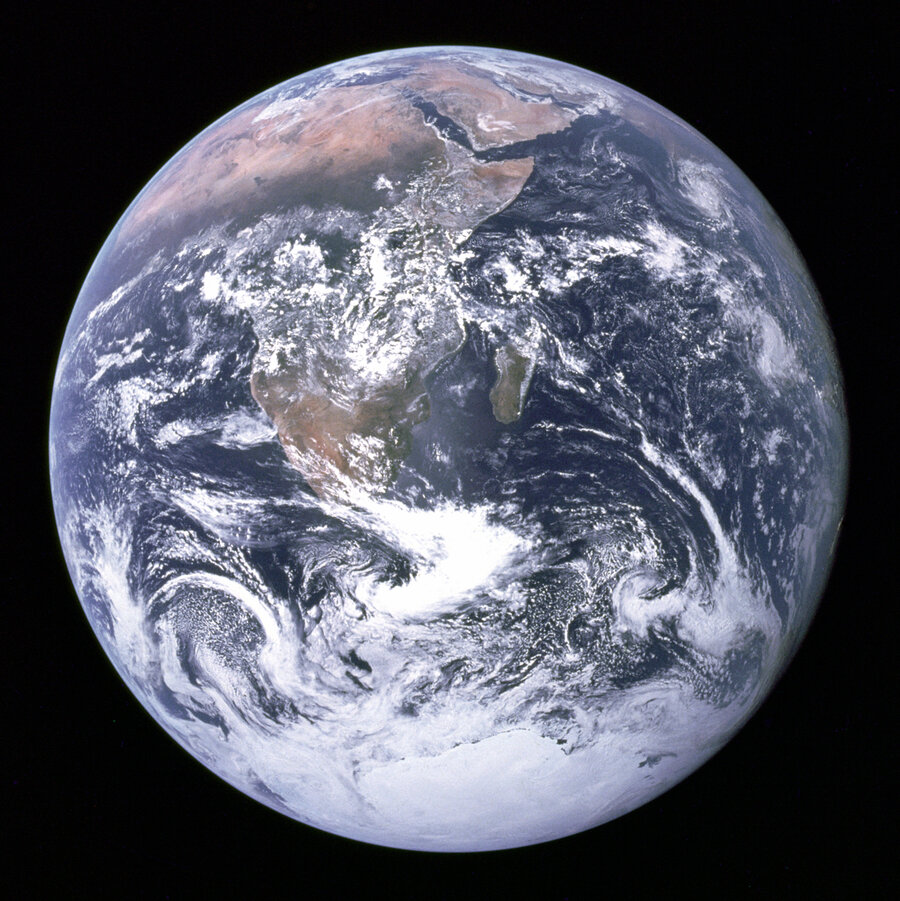
\includegraphics[width=\linewidth]{Grundlagen_Info/05_Datenintegritaet/Figures/bitrot_original.jpg}\\
            Original
        \end{minipage}
        \hspace{.05\textwidth}
        \begin{minipage}{.42\textwidth}
            \centering
            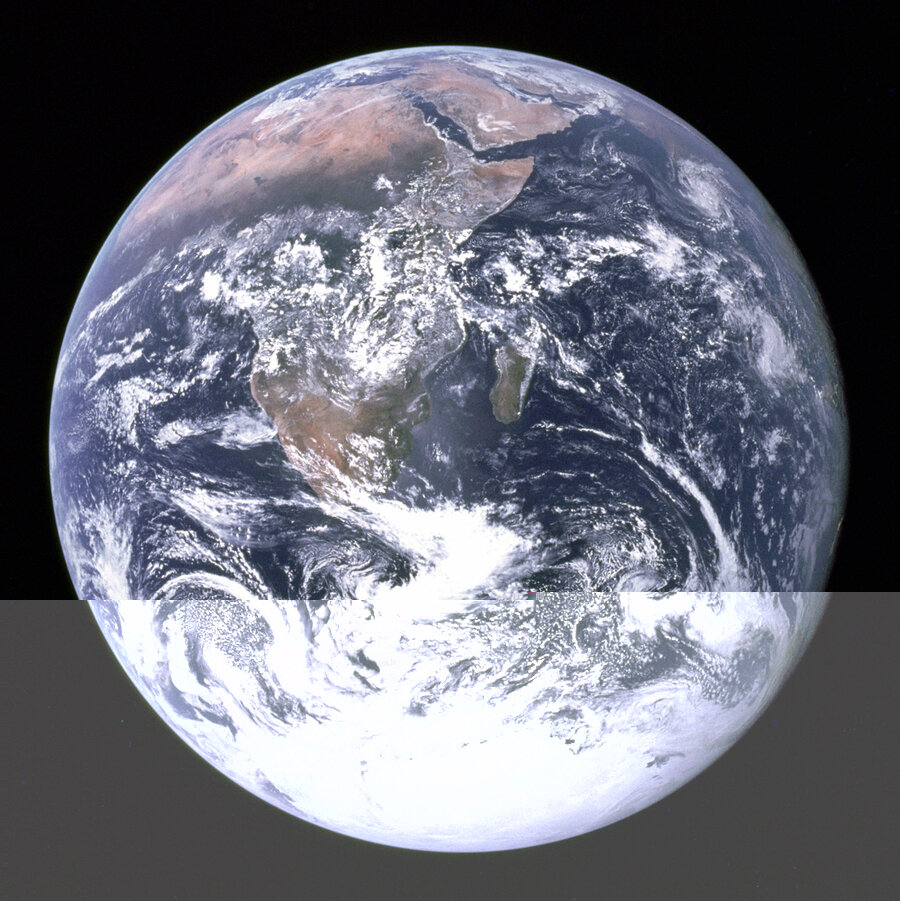
\includegraphics[width=\linewidth]{Grundlagen_Info/05_Datenintegritaet/Figures/bitrot.jpg}\\
            Nur 3 Bits gekippt
        \end{minipage}

        \vspace{2mm}
        \parbox{.8\textwidth}{\centering {\tiny Foto: NASA/Apollo 17 (\href{https://commons.wikimedia.org/wiki/File:The_Earth_seen_from_Apollo_17.jpg}{Wikimedia Commons}), gemeinfrei. Zum Weiterschauen: Tony \& Chelsea Northrup, \enquote{NAS Storage for Photos \& Video: PROTECT YOUR DATA!}, \url{https://www.youtube.com/watch?v=xvbnhCDfREk}}}
    \end{center}
\end{frame}

\begin{frame}{Mögliche Lösung: \glsentryshort{NAS} mit \glsentryshort{RAID}}
    \begin{center}
        \includegraphics[height=.45\textheight]{Grundlagen_Info/05_Datenintegritaet/Figures/NAS.png}
    \end{center}
    \begin{itemize}
        \item \gls{NAS}: Netzwerkgebundener Speicher
        \item \gls{RAID}: Redundante Anordnung unabhängiger Festplatten
        \item \textbf{Achtung:} \acrshort{RAID} ist kein Backup! Gelöschte, überschriebene, verschlüsselte (Ransomware) oder beschädigte Dateien landen sofort auf allen Platten $\rightarrow$ separates Backup (offline / extern)
    \end{itemize}
\end{frame}


\begin{frame}{\glsentryshort{RAID} 0}
    \begin{center}
        % RAID-Schemata (RAID 0, 1, 4, 5, 6) mit einheitlicher Notation:
% Buchstabe = Streifen, Zahl = Position im Streifen, p/q = Paritätsblock.
% Ersetzt die früheren Wikimedia-Grafiken (Cburnett), damit Skript, Folien
% und Aufgaben dieselben Namen und dieselbe Festplattennummerierung (ab 1) haben.
%
% Aufruf: \raidschema{<Festplatten>}{<Streifen>}{<Zeilen>}
%   <Zeilen>: eine Gruppe pro Streifen, darin pro Festplatte <Typ>/<Name>
%   Typ d = Datenblock, p = Paritätsblock P, q = Paritätsblock Q (RAID 6)
%   Beispiel RAID 4 mit drei Festplatten:
%   \raidschema{3}{2}{{d/A_1, d/A_2, p/A_p}, {d/B_1, d/B_2, p/B_p}}
%
% \providecommand, damit die Datei in Skript und Folien mehrfach
% eingebunden werden darf.
\providecommand{\raidschema}[3]{%
    \begin{tikzpicture}[
            raidblock/.style={draw, minimum width=1.2cm, minimum height=0.55cm, inner sep=1pt, font=\small},
            raidd/.style={raidblock, fill=blue!8},
            raidp/.style={raidblock, fill=orange!35},
            raidq/.style={raidblock, fill=red!25},
            raiddisk/.style={draw, thick, rounded corners=4pt, fill=gray!10}
        ]
        % Festplatten als Säulen, darunter die Nummer
        \foreach \j in {1,...,#1} {
                \draw[raiddisk] ({(\j-1)*1.9-0.8}, 0.5) rectangle ({(\j-1)*1.9+0.8}, {-(#2-1)*0.75-0.5});
                \node[font=\footnotesize, anchor=north] at ({(\j-1)*1.9}, {-(#2-1)*0.75-0.6}) {Festplatte \j};
            }
        % Blöcke: Zeile = Streifen, Spalte = Festplatte
        \foreach \row [count=\i] in {#3} {
                \foreach \typ/\lbl [count=\j] in \row {
                        \node[raid\typ] at ({(\j-1)*1.9}, {-(\i-1)*0.75}) {$\lbl$};
                    }
            }
    \end{tikzpicture}%
}

        \resizebox{!}{.36\textheight}{\raidschema{2}{4}{{d/A_1, d/A_2}, {d/B_1, d/B_2}, {d/C_1, d/C_2}, {d/D_1, d/D_2}}}
    \end{center}
    \begin{itemize}
        \item \textbf{Prinzip:} Striping (Daten werden in Blöcke aufgeteilt und auf die Festplatten verteilt)
        \item \textbf{Vorteil:} Hohe Geschwindigkeit
        \item \textbf{Nachteil:} Hohe Wahrscheinlichkeit für Datenverlust (kein Schutz)
        \item \textbf{Anwendung:} Temporäre / grosse Daten, z.B. Spiele
        \item \textbf{Kapazität:} $n$ Festplatten $\rightarrow$ $n$-fache Kapazität
    \end{itemize}
\end{frame}

\begin{frame}{\glsentryshort{RAID} 1}
    \begin{center}
        % RAID-Schemata (RAID 0, 1, 4, 5, 6) mit einheitlicher Notation:
% Buchstabe = Streifen, Zahl = Position im Streifen, p/q = Paritätsblock.
% Ersetzt die früheren Wikimedia-Grafiken (Cburnett), damit Skript, Folien
% und Aufgaben dieselben Namen und dieselbe Festplattennummerierung (ab 1) haben.
%
% Aufruf: \raidschema{<Festplatten>}{<Streifen>}{<Zeilen>}
%   <Zeilen>: eine Gruppe pro Streifen, darin pro Festplatte <Typ>/<Name>
%   Typ d = Datenblock, p = Paritätsblock P, q = Paritätsblock Q (RAID 6)
%   Beispiel RAID 4 mit drei Festplatten:
%   \raidschema{3}{2}{{d/A_1, d/A_2, p/A_p}, {d/B_1, d/B_2, p/B_p}}
%
% \providecommand, damit die Datei in Skript und Folien mehrfach
% eingebunden werden darf.
\providecommand{\raidschema}[3]{%
    \begin{tikzpicture}[
            raidblock/.style={draw, minimum width=1.2cm, minimum height=0.55cm, inner sep=1pt, font=\small},
            raidd/.style={raidblock, fill=blue!8},
            raidp/.style={raidblock, fill=orange!35},
            raidq/.style={raidblock, fill=red!25},
            raiddisk/.style={draw, thick, rounded corners=4pt, fill=gray!10}
        ]
        % Festplatten als Säulen, darunter die Nummer
        \foreach \j in {1,...,#1} {
                \draw[raiddisk] ({(\j-1)*1.9-0.8}, 0.5) rectangle ({(\j-1)*1.9+0.8}, {-(#2-1)*0.75-0.5});
                \node[font=\footnotesize, anchor=north] at ({(\j-1)*1.9}, {-(#2-1)*0.75-0.6}) {Festplatte \j};
            }
        % Blöcke: Zeile = Streifen, Spalte = Festplatte
        \foreach \row [count=\i] in {#3} {
                \foreach \typ/\lbl [count=\j] in \row {
                        \node[raid\typ] at ({(\j-1)*1.9}, {-(\i-1)*0.75}) {$\lbl$};
                    }
            }
    \end{tikzpicture}%
}

        \resizebox{!}{.36\textheight}{\raidschema{2}{4}{{d/A_1, d/A_1}, {d/B_1, d/B_1}, {d/C_1, d/C_1}, {d/D_1, d/D_1}}}
    \end{center}
    \begin{itemize}
        \item \textbf{Prinzip:} Mirroring (je zwei Festplatten bilden ein identisches Spiegelpaar)
        \item \textbf{Vorteil:} Hohe Ausfallsicherheit (pro Spiegelpaar kann eine Festplatte ausfallen)
        \item \textbf{Nachteil:} Nur halbe nutzbare Kapazität
        \item \textbf{Anwendung:} Wichtige Daten, z.B. Server
        \item \textbf{Kapazität:} $n$ Festplatten $\rightarrow$ $n/2$-fache Kapazität
    \end{itemize}
\end{frame}

\begin{frame}{Auftrag}{Skript \enquote{Datenintegrität}}
    \begin{itemize}
        \item \aufgabebox{1.26, 1.27 (\acrshort{RAID} 0 und 1)}
    \end{itemize}
\end{frame}


\begin{frame}{Parität mit \glsentryshort{XOR}}
    \begin{columns}
        \begin{column}{.35\textwidth}
            \begin{center}
                \begin{tabular}{ccc}
                    A & B & A $\oplus$ B \\\midrule
                    0 & 0 & 0            \\
                    0 & 1 & 1            \\
                    1 & 0 & 1            \\
                    1 & 1 & 0            \\
                \end{tabular}
            \end{center}
            \uncover<3->{
                \[
                    \begin{array}{r@{\;}l@{\quad}l}
                               & \mathtt{1011} & D_1                \\
                        \oplus & \mathtt{1100} & D_2                \\ \cline{1-2}
                               & \mathtt{0111} & D_1 \oplus D_2     \\
                        \oplus & \mathtt{0110} & D_3                \\ \cline{1-2}
                               & \mathtt{0001} & P \text{ (Parität)}
                    \end{array}
                \]
            }
        \end{column}
        \begin{column}{.6\textwidth}
            \begin{itemize}[<+->]
                \item \acrshort{XOR} (\enquote{exklusives Oder}): 1, wenn genau ein Bit 1 ist (Addition modulo 2)
                \item Bitfolgen werden Stelle für Stelle verknüpft
                \item Mehrere Blöcke: untereinander schreiben, mit dem Zwischenresultat weiterrechnen
                \item Fehlt ein Block, ergibt das \acrshort{XOR} der übrigen Blöcke mit \(P\) den fehlenden Block
            \end{itemize}
        \end{column}
    \end{columns}
\end{frame}


\begin{frame}{Auftrag}{Skript \enquote{Datenintegrität}}
    \begin{itemize}
        \item \aufgabebox{1.24, 1.25 (\acrshort{XOR})}
    \end{itemize}
\end{frame}


\begin{frame}{\glsentryshort{RAID} 5}
    \begin{center}
        % RAID-Schemata (RAID 0, 1, 4, 5, 6) mit einheitlicher Notation:
% Buchstabe = Streifen, Zahl = Position im Streifen, p/q = Paritätsblock.
% Ersetzt die früheren Wikimedia-Grafiken (Cburnett), damit Skript, Folien
% und Aufgaben dieselben Namen und dieselbe Festplattennummerierung (ab 1) haben.
%
% Aufruf: \raidschema{<Festplatten>}{<Streifen>}{<Zeilen>}
%   <Zeilen>: eine Gruppe pro Streifen, darin pro Festplatte <Typ>/<Name>
%   Typ d = Datenblock, p = Paritätsblock P, q = Paritätsblock Q (RAID 6)
%   Beispiel RAID 4 mit drei Festplatten:
%   \raidschema{3}{2}{{d/A_1, d/A_2, p/A_p}, {d/B_1, d/B_2, p/B_p}}
%
% \providecommand, damit die Datei in Skript und Folien mehrfach
% eingebunden werden darf.
\providecommand{\raidschema}[3]{%
    \begin{tikzpicture}[
            raidblock/.style={draw, minimum width=1.2cm, minimum height=0.55cm, inner sep=1pt, font=\small},
            raidd/.style={raidblock, fill=blue!8},
            raidp/.style={raidblock, fill=orange!35},
            raidq/.style={raidblock, fill=red!25},
            raiddisk/.style={draw, thick, rounded corners=4pt, fill=gray!10}
        ]
        % Festplatten als Säulen, darunter die Nummer
        \foreach \j in {1,...,#1} {
                \draw[raiddisk] ({(\j-1)*1.9-0.8}, 0.5) rectangle ({(\j-1)*1.9+0.8}, {-(#2-1)*0.75-0.5});
                \node[font=\footnotesize, anchor=north] at ({(\j-1)*1.9}, {-(#2-1)*0.75-0.6}) {Festplatte \j};
            }
        % Blöcke: Zeile = Streifen, Spalte = Festplatte
        \foreach \row [count=\i] in {#3} {
                \foreach \typ/\lbl [count=\j] in \row {
                        \node[raid\typ] at ({(\j-1)*1.9}, {-(\i-1)*0.75}) {$\lbl$};
                    }
            }
    \end{tikzpicture}%
}

        \resizebox{!}{.36\textheight}{\raidschema{4}{4}{{d/A_1, d/A_2, d/A_3, p/A_p}, {d/B_1, d/B_2, p/B_p, d/B_3}, {d/C_1, p/C_p, d/C_2, d/C_3}, {p/D_p, d/D_1, d/D_2, d/D_3}}}
    \end{center}
    \begin{itemize}
        \item \textbf{Prinzip:} Striping mit verteilter Parität (ein Paritätsblock pro Streifen, von Streifen zu Streifen auf einer anderen Festplatte)
        \item \textbf{Vorteil:} Gute Geschwindigkeit, Schutz bei Ausfall einer Festplatte
        \item \textbf{Nachteil:} Wiederherstellung bei Ausfall dauert lange
        \item \textbf{Anwendung:} Dateiserver, \gls{NAS}
        \item \textbf{Kapazität:} $n$ Festplatten $\rightarrow$ $(n-1)$-fache Kapazität
    \end{itemize}
\end{frame}

\begin{frame}{\glsentryshort{RAID} 6}
    \begin{center}
        % RAID-Schemata (RAID 0, 1, 4, 5, 6) mit einheitlicher Notation:
% Buchstabe = Streifen, Zahl = Position im Streifen, p/q = Paritätsblock.
% Ersetzt die früheren Wikimedia-Grafiken (Cburnett), damit Skript, Folien
% und Aufgaben dieselben Namen und dieselbe Festplattennummerierung (ab 1) haben.
%
% Aufruf: \raidschema{<Festplatten>}{<Streifen>}{<Zeilen>}
%   <Zeilen>: eine Gruppe pro Streifen, darin pro Festplatte <Typ>/<Name>
%   Typ d = Datenblock, p = Paritätsblock P, q = Paritätsblock Q (RAID 6)
%   Beispiel RAID 4 mit drei Festplatten:
%   \raidschema{3}{2}{{d/A_1, d/A_2, p/A_p}, {d/B_1, d/B_2, p/B_p}}
%
% \providecommand, damit die Datei in Skript und Folien mehrfach
% eingebunden werden darf.
\providecommand{\raidschema}[3]{%
    \begin{tikzpicture}[
            raidblock/.style={draw, minimum width=1.2cm, minimum height=0.55cm, inner sep=1pt, font=\small},
            raidd/.style={raidblock, fill=blue!8},
            raidp/.style={raidblock, fill=orange!35},
            raidq/.style={raidblock, fill=red!25},
            raiddisk/.style={draw, thick, rounded corners=4pt, fill=gray!10}
        ]
        % Festplatten als Säulen, darunter die Nummer
        \foreach \j in {1,...,#1} {
                \draw[raiddisk] ({(\j-1)*1.9-0.8}, 0.5) rectangle ({(\j-1)*1.9+0.8}, {-(#2-1)*0.75-0.5});
                \node[font=\footnotesize, anchor=north] at ({(\j-1)*1.9}, {-(#2-1)*0.75-0.6}) {Festplatte \j};
            }
        % Blöcke: Zeile = Streifen, Spalte = Festplatte
        \foreach \row [count=\i] in {#3} {
                \foreach \typ/\lbl [count=\j] in \row {
                        \node[raid\typ] at ({(\j-1)*1.9}, {-(\i-1)*0.75}) {$\lbl$};
                    }
            }
    \end{tikzpicture}%
}

        \resizebox{!}{.4\textheight}{\raidschema{5}{5}{{d/A_1, d/A_2, d/A_3, p/A_p, q/A_q}, {d/B_1, d/B_2, p/B_p, q/B_q, d/B_3}, {d/C_1, p/C_p, q/C_q, d/C_2, d/C_3}, {p/D_p, q/D_q, d/D_1, d/D_2, d/D_3}, {q/E_q, d/E_1, d/E_2, d/E_3, p/E_p}}}
    \end{center}
    \begin{itemize}
        \item \textbf{Prinzip:} Striping mit doppelter Parität (zwei Paritätsblöcke pro Streifen)
        \item \textbf{Vorteil:} Schutz bei Ausfall von zwei Festplatten
        \item \textbf{Nachteil:} Noch geringere nutzbare Kapazität, langsamere Schreibgeschwindigkeit
        \item \textbf{Anwendung:} Grosse Speicherlösungen mit hoher Sicherheit
        \item \textbf{Kapazität:} $n$ Festplatten $\rightarrow$ $(n-2)$-fache Kapazität
    \end{itemize}
\end{frame}

% Übersicht: alle RAID-Arten aus dem Skript mit je drei Streifen nebeneinander
% \raidbox{Breite}{Titel}{Schema}{Text}, ausserhalb des Frames definiert (# im Frame-Körper)
\providecommand{\raidbox}[4]{%
    \begin{minipage}[t]{#1}
        \centering
        \textbf{#2}\\[1mm]
        \resizebox{!}{.2\textheight}{#3}\\[1mm]
        \footnotesize #4
    \end{minipage}}
\begin{frame}{\glsentryshort{RAID}-Arten im Vergleich}
    % RAID-Schemata (RAID 0, 1, 4, 5, 6) mit einheitlicher Notation:
% Buchstabe = Streifen, Zahl = Position im Streifen, p/q = Paritätsblock.
% Ersetzt die früheren Wikimedia-Grafiken (Cburnett), damit Skript, Folien
% und Aufgaben dieselben Namen und dieselbe Festplattennummerierung (ab 1) haben.
%
% Aufruf: \raidschema{<Festplatten>}{<Streifen>}{<Zeilen>}
%   <Zeilen>: eine Gruppe pro Streifen, darin pro Festplatte <Typ>/<Name>
%   Typ d = Datenblock, p = Paritätsblock P, q = Paritätsblock Q (RAID 6)
%   Beispiel RAID 4 mit drei Festplatten:
%   \raidschema{3}{2}{{d/A_1, d/A_2, p/A_p}, {d/B_1, d/B_2, p/B_p}}
%
% \providecommand, damit die Datei in Skript und Folien mehrfach
% eingebunden werden darf.
\providecommand{\raidschema}[3]{%
    \begin{tikzpicture}[
            raidblock/.style={draw, minimum width=1.2cm, minimum height=0.55cm, inner sep=1pt, font=\small},
            raidd/.style={raidblock, fill=blue!8},
            raidp/.style={raidblock, fill=orange!35},
            raidq/.style={raidblock, fill=red!25},
            raiddisk/.style={draw, thick, rounded corners=4pt, fill=gray!10}
        ]
        % Festplatten als Säulen, darunter die Nummer
        \foreach \j in {1,...,#1} {
                \draw[raiddisk] ({(\j-1)*1.9-0.8}, 0.5) rectangle ({(\j-1)*1.9+0.8}, {-(#2-1)*0.75-0.5});
                \node[font=\footnotesize, anchor=north] at ({(\j-1)*1.9}, {-(#2-1)*0.75-0.6}) {Festplatte \j};
            }
        % Blöcke: Zeile = Streifen, Spalte = Festplatte
        \foreach \row [count=\i] in {#3} {
                \foreach \typ/\lbl [count=\j] in \row {
                        \node[raid\typ] at ({(\j-1)*1.9}, {-(\i-1)*0.75}) {$\lbl$};
                    }
            }
    \end{tikzpicture}%
}

    \centering
    \raidbox{.22\textwidth}{\acrshort{RAID} 0}{\raidschema{2}{3}{{d/A_1, d/A_2}, {d/B_1, d/B_2}, {d/C_1, d/C_2}}}{Kapazität $n$\\kein Schutz}\hfill
    \raidbox{.22\textwidth}{\acrshort{RAID} 1}{\raidschema{2}{3}{{d/A_1, d/A_1}, {d/B_1, d/B_1}, {d/C_1, d/C_1}}}{Kapazität $n/2$\\Spiegelung}\hfill
    \raidbox{.4\textwidth}{\acrshort{RAID} 4}{\raidschema{4}{3}{{d/A_1, d/A_2, d/A_3, p/A_p}, {d/B_1, d/B_2, d/B_3, p/B_p}, {d/C_1, d/C_2, d/C_3, p/C_p}}}{Kapazität $n-1$\\1 Platte darf ausfallen}

    \vspace{4mm}
    \raidbox{.4\textwidth}{\acrshort{RAID} 5}{\raidschema{4}{3}{{d/A_1, d/A_2, d/A_3, p/A_p}, {d/B_1, d/B_2, p/B_p, d/B_3}, {d/C_1, p/C_p, d/C_2, d/C_3}}}{Kapazität $n-1$\\1 Platte darf ausfallen}\hfill
    \raidbox{.45\textwidth}{\acrshort{RAID} 6}{\raidschema{5}{3}{{d/A_1, d/A_2, d/A_3, p/A_p, q/A_q}, {d/B_1, d/B_2, p/B_p, q/B_q, d/B_3}, {d/C_1, p/C_p, q/C_q, d/C_2, d/C_3}}}{Kapazität $n-2$\\2 Platten dürfen ausfallen}
\end{frame}

\begin{frame}{Auftrag}{Skript \enquote{Datenintegrität}}
    \begin{itemize}
        \item \aufgabebox{1.28--1.31 (\acrshort{RAID} 5 und 6)}
    \end{itemize}
\end{frame}


\begin{frame}{\glsentryshort{RAID} ist kein Backup}
    \begin{columns}[T,onlytextwidth]
        \column{.48\textwidth}
        \textbf{\acrshort{RAID} schützt vor \dots}
        \begin{itemize}
            \item Ausfall einer Festplatte (\acrshort{RAID} 6: zwei)
            \item Stillstand: das System läuft weiter
        \end{itemize}
        \column{.48\textwidth}
        \textbf{\acrshort{RAID} schützt \textit{nicht} vor \dots}
        \begin{itemize}[<+->]
            \item versehentlichem Löschen / Überschreiben
            \item Ransomware
            \item Diebstahl, Brand, Wasserschaden
            \item \textit{bit rot}, das unbemerkt bleibt
        \end{itemize}
    \end{columns}
    \vspace{4mm}
    \begin{center}
        \only<5>{Jede Änderung landet sofort auf \textit{allen} Festplatten $\rightarrow$ es braucht eine \textbf{separate} Kopie: ein \textbf{Backup}.}
    \end{center}
\end{frame}

\begin{frame}{Die 3-2-1-Regel}
    \begin{center}
        \resizebox{.95\textwidth}{!}{% 3-2-1-Backup-Regel: 3 Kopien, auf 2 verschiedenen Medien, davon 1 ausser Haus.
% Wird im Skript (Abschnitt Backup) und auf den RAID-Folien verwendet.
\begin{tikzpicture}[
        copy/.style={draw, rounded corners, thick, minimum width=3.2cm, minimum height=1.5cm, align=center, font=\small},
        zone/.style={draw, dashed, rounded corners, inner sep=8pt},
        lbl/.style={font=\footnotesize\bfseries, anchor=south west}
    ]
    % Zuhause: Original und erste Kopie auf einem anderen Medium
    \node[copy, fill=blue!10]   (orig)  at (0,0)   {\faLaptop\\[2pt] Original\\ \footnotesize Laptop (SSD)};
    \node[copy, fill=green!12]  (copy1) at (4,0)   {\faHdd\\[2pt] Kopie 1\\ \footnotesize externe Festplatte / \acrshort{NAS}};
    % Ausser Haus: zweite Kopie
    \node[copy, fill=orange!15] (copy2) at (9.8,0)   {\faCloud\\[2pt] Kopie 2\\ \footnotesize Cloud / Festplatte bei Verwandten};

    \node[zone, fit=(orig)(copy1)]  (home) {};
    \node[zone, fit=(copy2)]        (away) {};
    \node[lbl] at (home.north west) {Zuhause};
    \node[lbl] at (away.north west) {Ausser Haus};

    \draw[-latex, thick] (orig) -- (copy1);
    \draw[-latex, thick] (copy1) -- (copy2);

    % Die drei Regeln unter der Grafik
    \node[font=\small, align=center] at (4.9,-1.9)
    {\textbf{3} Kopien \quad\textperiodcentered\quad auf \textbf{2} verschiedenen Medien \quad\textperiodcentered\quad davon \textbf{1} ausser Haus};
\end{tikzpicture}
}
    \end{center}
    \begin{itemize}
        \item Backups automatisch und regelmässig erstellen, ältere Versionen aufbewahren
        \item Wiederherstellung testen -- erst dann weiss man, dass das Backup funktioniert
    \end{itemize}
\end{frame}

\begin{frame}{Erweiterung: die 3-2-1-1-0-Regel}
    \begin{center}
        \resizebox{.95\textwidth}{!}{% 3-2-1-1-0-Backup-Regel: Erweiterung der 3-2-1-Regel (tikz_backup_321.tex) um
% 1 Kopie offline bzw. unveränderlich und 0 Fehler beim Wiederherstellungstest.
% Wird im Skript (Ende Abschnitt Backup) und auf den RAID-Folien verwendet.
\begin{tikzpicture}[
        copy/.style={draw, rounded corners, thick, minimum width=3.2cm, minimum height=1.5cm, align=center, font=\small},
        zone/.style={draw, dashed, rounded corners, inner sep=8pt},
        lbl/.style={font=\footnotesize\bfseries, anchor=south west},
        % Kreis mit Ziffer und Beschriftung für die Zeile der fünf Regeln
        rule/.style={circle, draw, thick, minimum size=7mm, inner sep=0pt, font=\bfseries}
    ]
    % Gleiche Anordnung wie bei der 3-2-1-Regel
    \node[copy, fill=blue!10]   (orig)  at (0,0)   {\faLaptop\\[2pt] Original\\ \footnotesize Laptop (SSD)};
    % Kopie 1 ist zusätzlich offline: nur während des Backups angeschlossen
    \node[copy, fill=green!12, line width=1.6pt] (copy1) at (4,0) {\faHdd\ \faUnlink\\[2pt] Kopie 1 (offline)\\ \footnotesize externe Festplatte, abgehängt};
    \node[copy, fill=orange!15] (copy2) at (9.8,0) {\faCloud\\[2pt] Kopie 2\\ \footnotesize Cloud / Festplatte bei Verwandten};

    \node[zone, fit=(orig)(copy1)]  (home) {};
    \node[zone, fit=(copy2)]        (away) {};
    \node[lbl] at (home.north west) {Zuhause};
    \node[lbl] at (away.north west) {Ausser Haus};

    \draw[-latex, thick] (orig) -- (copy1);
    \draw[-latex, thick] (copy1) -- (copy2);

    % Test-Wiederherstellung aus dem Backup zurück aufs Original
    \draw[-latex, thick, dashed, green!50!black] (copy2.north) to[out=150, in=30]
        node[above, font=\footnotesize, text=black] {\faCheckCircle\ Wiederherstellung testen: \textbf{0} Fehler} (orig.north);

    % Die fünf Regeln unter der Grafik
    \foreach \n/\txt [count=\i from 0] in {3/Kopien, 2/Medien, 1/ausser Haus, 1/offline oder\\unveränderlich, 0/Fehler beim\\Test} {
        \node[rule] (r\i) at (\i*2.45,-2.1) {\n};
        \node[font=\footnotesize, align=center, anchor=north] at (r\i.south) {\txt};
    }
\end{tikzpicture}
}
    \end{center}
    \begin{itemize}
        \item \textbf{1} Kopie offline (nur beim Backup angeschlossen) oder unveränderlich: Ransomware kann sie nicht verschlüsseln
        \item \textbf{0} Fehler beim regelmässigen Test der Wiederherstellung
    \end{itemize}
\end{frame}

\begin{frame}{Auftrag}{Skript \enquote{Datenintegrität}}
    \begin{itemize}
        \item \aufgabebox{1.32, 1.33 (Backup)}
    \end{itemize}
\end{frame}
